\section{Introduction}
\IEEEPARstart{A}{utonomous} tank trucks are emerging as a safety-critical carrier for hazardous-liquid logistics, where the planning and control problem is fundamentally different from that of ordinary passenger cars or rigid-load trucks. Hazardous-material road transport continues to rely heavily on liquid tank trucks, while accident investigations indicate that tanker rollovers are frequent in severe hazardous-material transportation accidents \cite{qianyuyan2023,authority_tank_truck2022}. Such events are particularly destructive because leakage, fire, explosion, and environmental pollution can follow the initial vehicle instability; the 2020 Wenling liquefied-petroleum-gas tanker accident is a representative case \cite{wenling_accident2022}. The causes of tank-truck rollover can be summarized into three coupled aspects: vehicle--liquid dynamics, single-vehicle information limitations, and human or maneuvering errors. Liquid tanks usually operate under non-full filling conditions because of expansion and pressure constraints, which makes liquid sloshing unavoidable in practical transportation \cite{biaozhunR00052011}. Meanwhile, a single vehicle has limited perception range and often lacks sufficient knowledge of road topology, surrounding-vehicle intention, and downstream traffic evolution. Rollover prevention is therefore not only a vehicle-stability problem, but also a predictive planning problem.

The rollover risk of a tank truck is strongly shaped by vehicle--liquid coupling. Existing studies usually explain this coupling through two mechanisms: quasi-static migration of the liquid centroid and transient sloshing impact. The former changes the equivalent center of mass and roll moment under lateral acceleration, while the latter introduces additional lateral force and roll moment during transient maneuvers such as lane changes and obstacle avoidance \cite{maohaijian2021fsi,wangxiaorun2022lateralacc,wanying2020antirolover}. For modeling, quasi-static and CFD methods are useful for mechanism analysis and offline calibration, whereas mechanical-equivalent models are more suitable for online planning and control because they retain the dominant sloshing dynamics with much lower computational cost \cite{yuzhixin2018mpc,zhaoweiqiang2019semitrailer,Komasa2023observing,KomasaQi2025AntiRollover_TITS}. For articulated or semi-trailer tank trucks, the tractor--trailer articulation further couples yaw, roll, lateral motion, and liquid sloshing, so the simplified model must preserve the dominant rollover modes while remaining tractable for real-time optimization \cite{zongchangfu2014identification}.

Rollover-oriented active safety has been studied from both planning and control perspectives. In motion planning, rollover risk is commonly described by load-transfer, rollover-time, or stability-margin indices and then embedded into search, sampling, or optimization-based trajectory generation \cite{jin2021heavytruck,rasekhipour2017pfmpc,li2019rollover}. In control, active steering, differential braking, and MPC-related methods have been used to suppress roll motion and reduce LTR when the vehicle approaches a dangerous boundary \cite{zhao2019hinfty,Reviewer2_SunWencai2022,weixing2023_antirollover}. These studies provide important foundations for tank-truck stability protection. However, most vehicle-side methods are short-horizon and reactive. They can mitigate a risky maneuver after the maneuver has already been selected, but they do not sufficiently prevent interaction-induced risks from forming in the first place.

This limitation becomes clearer when viewed against the broader development of autonomous-driving decision-making. Since the DARPA Urban Challenge, modular autonomous-driving systems have typically followed a perception--prediction--decision--planning--control pipeline \cite{ferguson2008urban}. In interactive traffic, however, surrounding vehicles respond to the ego decision, so prediction and decision should be coupled. Explicit interaction methods evaluate surrounding-vehicle reactions under candidate ego behaviors \cite{cunningham2015mpdm,ding2022epsilon}, while contingency, game-theoretic, and risk-aware methods reason over uncertain future scenarios and multi-agent influence \cite{da2022reactivesafety,li2020gametheorytits,li2023marc}. End-to-end and generative planning methods further attempt to learn joint representations for prediction and planning from structured or raw perception inputs \cite{hu2022uniAD,DiffusionPlanner2025}. Nevertheless, most of these methods are designed for ordinary vehicles and general traffic safety; rollover-induced constraints, liquid sloshing, and articulated heavy-vehicle dynamics are rarely included in the decision loop.

Vehicle--road--cloud integration offers a complementary way to address the long-horizon nature of interaction-induced rollover risk. Cloud-control systems can aggregate road topology, roadside perception, vehicle uploads, map services, traffic-management information, and cloud computation to extend the perception and prediction horizon beyond a single vehicle \cite{likeqiang2020cloudcontrol,icv2023whiteroadcloud}. Recent V2X and cloud-based driving studies show that cooperative perception, prediction, and planning can improve the safety and efficiency of connected autonomous vehicles \cite{Huang2025V2X,Gao2025V2X}. Existing vehicle--cloud decision architectures can be roughly interpreted as three types: V2X-assisted vehicle-side autonomy, vehicle--cloud hierarchical control, and cloud-centered global control. Cloud-centered coordination can optimize traffic flow, ramp merging, and multi-vehicle behavior at a larger scale, but it usually depends on high penetration, reliable communication, and sufficient infrastructure deployment \cite{Yang2025CloudBased,Wang2025Cooperative}. For mixed traffic and low-penetration scenarios, vehicle--cloud hierarchical control is more practical because the cloud provides low-frequency predictive guidance while the vehicle retains high-frequency safety closure. Its effectiveness, however, depends on whether the vehicle can absorb cloud guidance under delay, jitter, packet loss, local perception updates, and actuator constraints \cite{xionglu2024_CVIS_survay,xuqing2021unreliable,wang2021platoonmpc}.

The above literature suggests three gaps for autonomous tank-truck rollover prevention. First, tank-truck studies have deeply investigated vehicle--liquid dynamics and short-horizon anti-rollover control, but they rarely use wide-area cloud information to avoid interaction-induced rollover triggers before they become local emergencies. Second, cloud-control and V2X studies improve prediction and cooperative planning, but they usually target ordinary vehicles, traffic efficiency, or general collision safety rather than heavy articulated tank trucks with liquid sloshing and rollover constraints. Third, system-architecture studies provide useful reference models for connected-vehicle systems and cyber-physical transportation systems, but they still need to be connected with concrete planning and control algorithms that define what the cloud predicts, what the vehicle replans, and what the controller must guarantee \cite{qixiaojing2026mbsose}. A practical autonomous tank-truck system therefore requires a nested multi-time-scale formulation: the cloud should anticipate induced risks through long-horizon interaction prediction, the vehicle-side planner should provide degraded-safety fallback under abrupt local hazards or cloud-reference infeasibility, and the high-frequency controller should suppress state risks caused by roll motion and liquid sloshing.

This paper proposes a vehicle--cloud collaborative predictive planning and anti-rollover control framework for autonomous tank trucks. The cloud-side module represents highway traffic as a directed road graph, uses a Graphflow-based interactive prediction model as a learned world model, and trains a reinforcement-learning policy to generate long-horizon speed and lane-change decisions. The resulting decision is converted into a rollover-aware reference trajectory rather than a direct control command. The vehicle-side emergency planning module treats this reference as an initial guide, screens local multimodal interaction risks, and performs dual-scenario contingency replanning when sudden hazards or cloud-trajectory infeasibility are detected. Finally, a high-frequency multi-constraint MPC tracks the selected trajectory while coordinating steering, differential braking, and desired speed to constrain liquid sloshing, equivalent LTR, actuator limits, and tracking error.

\begin{figure*}[t]
  \centering
  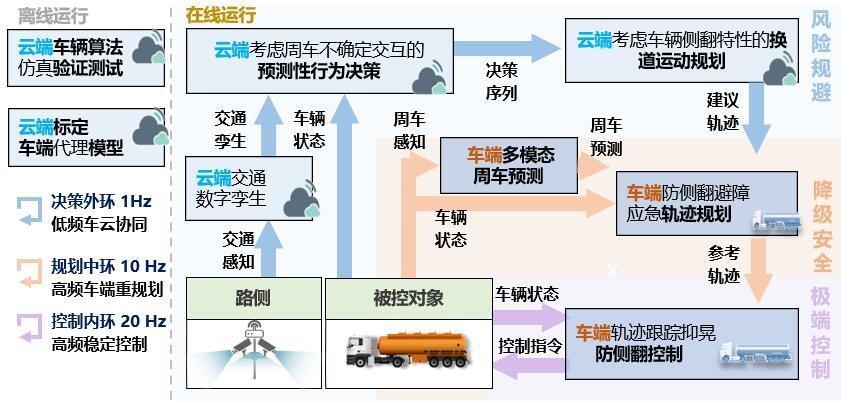
\includegraphics[width=0.92\textwidth]{fig/chap2/safe_arch.jpg}
  \caption{Vehicle--cloud collaborative predictive planning and anti-rollover control framework. The cloud side provides long-horizon predictive planning, the vehicle-side planner provides emergency trajectory replanning, and the high-frequency controller enforces trajectory tracking, sloshing suppression, and rollover prevention.}
  \label{fig:vc_framework}
\end{figure*}
% TODO: Redraw Fig. \ref{fig:vc_framework} in English for the final submission. The figure should show cloud-side Graphflow prediction and decision-making, vehicle-side emergency planning, high-frequency MPC, information upload/download, and fallback under communication uncertainty.

The overall information flow is shown in Fig.~\ref{fig:vc_framework}. The cloud side receives the ego state, surrounding traffic graph, road topology, and transportation-task information, and outputs a long-horizon driving decision and a rollover-aware reference trajectory. The vehicle-side planner receives the cloud trajectory, local perception, and ego state, and outputs a locally feasible emergency trajectory when needed. The controller receives the selected reference trajectory and measured or estimated vehicle--liquid states, and outputs steering, differential braking, and speed commands. This structure follows the principle that the cloud reduces the probability of entering dangerous interactions, the vehicle-side planner preserves feasibility when the cloud guide is no longer safe, and the controller forms the final anti-rollover safety layer.

The main contributions are summarized as follows:
\begin{itemize}
  \item A vehicle--cloud collaborative predictive planning and anti-rollover control framework is proposed for autonomous tank trucks, integrating long-horizon cloud-side risk anticipation with vehicle-side real-time stability protection.
  \item A Graphflow-based cloud-side predictive planning module is developed to represent large-scale highway traffic as a directed graph, model long-horizon stochastic interaction, and support reinforcement-learning decision-making through a learned world model.
  \item A vehicle-side planning and high-frequency control strategy is formulated by combining dual-scenario contingency replanning, coupled liquid--vehicle dynamics, and multi-constraint MPC for trajectory tracking, sloshing suppression, and rollover prevention.
  \item The proposed method is validated through traffic simulation, high-fidelity vehicle--liquid co-simulation, and scaled tank-truck experiments.
\end{itemize}

The remainder of this paper is organized as follows. Section~II formulates the vehicle--cloud collaborative anti-rollover problem. Section~III presents the cloud-side predictive planning method. Section~IV introduces vehicle-side emergency planning and high-frequency anti-rollover control. Section~V reports simulation and experimental validation. Section~VI concludes the paper, and the Appendix provides additional modeling and implementation details.
